%-------------------------------------------------------------------------------------

\documentclass[]{beamer}
\usepackage[utf8x]{inputenc}
\usepackage{hyperref}
\usepackage{fontawesome}
\usepackage{graphicx}
\usepackage[T2A]{fontenc}
\usepackage[serbian]{babel}
\usepackage{booktabs}
\usepackage{hyperref}

%-------------------------------------------------------------------------------------

\mode<presentation>
{
    \usetheme[progressbar=foot,numbering=fraction,background=light]{Boadilla} 
    \usecolortheme{seahorse}
    \usefonttheme{default}
    \setbeamertemplate{navigation symbols}{}
    \setbeamertemplate{caption}[numbered]
}

\setbeamertemplate{footline}
{
  \hbox{\begin{beamercolorbox}[wd=1\paperwidth,ht=2.25ex,dp=2ex,right]{framenumber}%
      \usebeamerfont{framenumber}\insertframenumber{} / \inserttotalframenumber\hspace*{2ex}
    \end{beamercolorbox}}%
  \vskip0pt%
}

%-------------------------------------------------------------------------------------

\usepackage{minted}

%-------------------------------------------------------------------------------------

\title[]{Симулација физике у 2D простору}
\author[magley] {Лазар Магазин SV 25/2020}
\institute[FTN] {Факултет техничких наука \\ Универзитет у Новом Саду}

%-------------------------------------------------------------------------------------

\begin{document}

\begin{frame}
    \titlepage
\end{frame}

%-------------------------------------------------------------------------------------

\begin{frame}{Садржај}
    \tableofcontents
\end{frame}

%-------------------------------------------------------------------------------------

\AtBeginSection{}
\section{Увод}
\begin{frame}{Увод}
    Задатак:
    \begin{itemize}
    \item моделовати неке од физичких закона кретања
    \item за крута тела
    \item у дводимензионом простору
    \end{itemize}
    Проблеми:
    \begin{itemize}
    \item како представити физичке величине
    \item како представити физички систем
    \item како решити диференцијалне једначине
    \item како детектовати сударе тела
    \item како ограничити кретање тела
    \item како реаговати нумеричке грешке
    \end{itemize}
\end{frame}

%-------------------------------------------------------------------------------------

\section{Физичке величине - скалар, вектор, матрица}
\begin{frame}[fragile]{Физичке величине}
    \textbf{Скалари}: маса, момент инерције, коефицијенти - \mintinline{c++}{double} \\
    \textbf{Вектори}: положај, брзина, импулс, сила
    
    \begin{minted}{c++}
    struct Vec2 {
        double x, y;
    }; // utility/mathutil.h
    \end{minted}
    
    \textbf{Матрица}: ротациона матрица
    
    \begin{minted}{c++}
    struct Mat2x2 {
        double m00, m10, m01, m11;
    }; // utility/mathutil.h
    \end{minted}
    
\end{frame}

\begin{frame}[fragile]{Физички систем - облик и тело}
    \textbf{Облик} - особине крутог тела ван простора
    
    \begin{minted}{c++}
    struct Shape {
        double radius;                // За кругове
        std::vector<Vec2> vert, norm; // За многоуглове
    }; // naphy/shape.х
    \end{minted}
    
    \textbf{Тело} - облик у простору
    
    \begin{minted}{c++}
    struct PhysBody {
        Shape shape;
        Vec2 pos, vel, force;
        double ang, angvel, torque;
        double m, I, m_inv, I_inv;
    }; // naphy/physbody.h
    \end{minted}
    
\end{frame}

\begin{frame}[fragile]{Физички систем - сцена}
    \textbf{Сцена} - физички систем
    
    \begin{minted}{c++}
    struct PhysScene {
        std::vector<PhysBody> bodies;   // Тела
        std::vector<Arbtier> arbiters;  // Арбитери
        std::vector<Spring> springs;    // Опруге
    }; // naphy/physscene.h
    \end{minted}
    
\end{frame}

%-------------------------------------------------------------------------------------

\section{Диференцијалне једначине}
\begin{frame}[fragile]{Диференцијалне једначине}
    Једначине кретања (2. Њутнов закон) \\
    \textbf{Симплектички Ојлеров} метод

    \begin{minted}{c++}
    vel += acc * dt; // Експлицитно
    pos += vel * dt; // Имплицитно
    \end{minted}
    
    Друге методе (вишекорачне Адамс-Башфорта) прецизније али исте стабилности \\
    Симпл. Ојлер је углавном довољан*
\end{frame}

%-------------------------------------------------------------------------------------

\section{Детекција колизије}
\begin{frame}[fragile]{Детекција колзије}
    \textbf{круг-круг} - поређење растојање са збиром полупречника \\
    \textbf{круг-многоугао} - \textit{SAT}: нормала минималног пресека пројекција \\
    \textbf{многоугао-многоугао} - \textit{SAT} \\
    \\
    Оптимизација - екстремна тачка (\textit{support point}) \\
    Исецање многоуглова - \textit{Sutherland-Hodgman} алгоритам \\
\end{frame}

\begin{frame}[fragile]{Детекција колзије - арбитер}
    \textbf{Арбитер} - све информације о колизији између два тела
    \begin{minted}{c++}
    struct Arbiter {
        PhysBody *A, *B;
        double depth;
        Vec2 normal;
        std::vector<Vec2> contact;
    }; // naphy/arbiter.h
    \end{minted}
\end{frame}

%-------------------------------------------------------------------------------------

\section{Ограничења}
\begin{frame}{Ограничења (constraints)}
    $C(x) = 0$ \\
    Ограничавамо положај и оријентацију: $C(x) = C(p, r)$ \\
    Ограничење упада - потребна су два тела: $C(x) = C(p_1, r_1, p_2, r_2)$ \\
    \\
    Решавање по изводу: $C(x) = 0 \Rightarrow \dot{C}(x) = 0$
\end{frame}


\begin{frame}{Ограничења - non-penetration constraint}
    Ако $\dot{C} \neq 0$, потребно је деловати на тела силом
    \begin{figure}[htp]
        \centering
        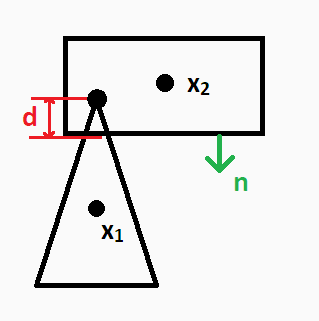
\includegraphics[width=6cm]{img_01.png}
    \end{figure}
    $C(p_1, r_1, p_2, r_2) = d = n\cdot(x_2 - x_1)$
\end{frame}

\begin{frame}{Ограничења - non-penetration constraint}
    $C = (x_2 - x_1) \cdot n$ \\
    $\dot{C} = \frac{d}{dt}(x_2 - x_1) \cdot n + (x_2 - x_1)\cdot\frac{d}{dt}n$ \\
    $= (\frac{d}{dt}x_2 - \frac{d}{dt}x_1)\cdot n + (x_2 - x_1)\cdot\frac{d}{dt}n$ \\
    $= (v_2+\omega_2\times r_2-v_1-\omega_1\times r_1)n + (x_2 - x_1)\cdot\frac{d}{dt}n$ \\
    \\
    Интересује нас само брзина, па се $(x_2 - x_1)\cdot\frac{d}{dt}n$ игнорише: \\
    $= (v_2+\omega_2\times r_2-v_1-\omega_1\times r_1)n$ \\
    $= v_2 n + (\omega_2 \times r_2)n - v_1 n - (\omega_1 \times r_1)n$ \\
    \\
    Важи особина мешовитог производа: $(a \times b)\cdot c = a \cdot (b \times c):$ \\
    $= v_2 n + \omega_2 (r_2 \times n) - v_1 n - \omega_1 (r_1 \times n)$ \\
    $= \begin{bmatrix} -n & -(r_1 \times n) & n & (r_2 \times n)\end{bmatrix}
        \begin{bmatrix} v_1 & \omega_1 & v_2 & \omega_2 \end{bmatrix} $ \\
\end{frame}

\begin{frame}{Ограничења - non-penetration constraint}
    $\dot{C} = \begin{bmatrix} -n & -(r_1 \times n) & n & (r_2 \times n)\end{bmatrix}
        \begin{bmatrix} v_1 & \omega_1 & v_2 & \omega_2 \end{bmatrix}
    = J \cdot V $ \\
    
    Ако $\dot{C} \neq 0$, онда постоји $\Delta V$ такво да је $\dot{C} = J(V+\Delta V) = 0$ \\
    Занима нас импулс* ($p = m \Delta v, L = r \times p$)\\
    $\Delta V = 
    \begin{bmatrix}
        -\frac{p}{m_1} & -\frac{r_1 \times p}{I_1} & \frac{p}{m_2} & \frac{r_2 \times p}{I_2}
    \end{bmatrix}$ \\
    Знамо правац импулса ($n$), интензитет је непознат: $p = \lambda n$ \\
    $
    \Delta V = 
    \begin{bmatrix}
        -\frac{p}{m_1} & -\frac{r_1 \times p}{I_1} & \frac{p}{m_2} & \frac{r_2 \times p}{I_2}
    \end{bmatrix}
    = \\
    \begin{bmatrix}
        -\frac{\lambda n}{m_1} & -\frac{r_1 \times \lambda n}{I_1} & \frac{\lambda n}{m_2} & \frac{r_2 \times \lambda n}{I_2}
    \end{bmatrix}
    = \\
    \lambda \begin{bmatrix} -\frac{n}{m_1} & -\frac{r_1 \times n}{I_1} & \frac{n}{m_2} & \frac{r_2 \times n}{I_2}\end{bmatrix} 
    $ \\ 
    Решити ограничење значи пронаћи $\lambda$ за које $J(V + \Delta V) = 0$ \\
    * зашто импулс?
\end{frame}

%-------------------------------------------------------------------------------------

\section{Секвенцијални импулси}

\begin{frame}{Секвенцијални импулси}
    Зашто импулс? \\
    \\
    Једна колизија $\Rightarrow$ један арбитер $\Rightarrow$ једно ограничење $\Rightarrow$ једно $\lambda$ \\
    Више колизија у једном тренутку $\Rightarrow$ више $\lambda$ које треба решити \\
    Систем ограничења \\
    \\
    (А) Глобално решавање система ограничења \\
    (Б) Итеративно решавање система ограничења \\
    \\
    \textbf{Секвенцијални импулси} - итеративни метод
\end{frame}

\begin{frame}{Секвенцијални импулси}
    $ \Delta V =  \lambda 
    \begin{bmatrix} 
        -\frac{n}{m_1} & -\frac{r_1 \times n}{I_1} & \frac{n}{m_2} & \frac{r_2 \times n}{I_2}
    \end{bmatrix} \\ $
    Извучемо масе: \\
    \\\
    $
    \Delta V = \lambda 
    \begin{bmatrix}
        \frac{1}{m_1} & 0 & 0 & 0 \\
        0 & \frac{1}{I_1} & 0 & 0 \\
        0 & 0 & \frac{1}{m_2} & 0 \\
        0 & 0 & 0 & \frac{1}{I_2} \\
    \end{bmatrix}
    \begin{bmatrix}
        -n \\
        -(r_1 \times n) \\
        n \\
        (r_2 \times n)
    \end{bmatrix}
    = \lambda M^{-1}J^T
    $ \\
    \\
    \\
    $J(V + \Delta V) = 0$ \\
    $\Rightarrow \lambda = -\frac{JV}{J M^{-1} J^T}$\\
\end{frame}

\begin{frame}[fragile]{Секвенцијални импулси}
    $\lambda = -\frac{JV}{J M^{-1} J^T},\quad p = m \Delta v = \lambda n $
    \begin{minted}{c++}
// JV = C' = dv * n
Vec2 dv = (B->vel + cross(B->angvel, r2))
         -(A->vel + cross(A->angvel, r1));
Vec2 dvn = dot(dv, n);
// J M^-1 J^T
double m = (A->m_inv + r1n * r1n * A->I_inv)
          +(B->m_inv + r2n * r2n * B->I_inv);
// p = lambda * n
Vec2 impulse = (-dvn / m) * n;
A->vel -= impulse * A->m_inv;
B->vel += impulse * B->m_inv;
// naphy/arbiter.cpp :: solve(), apply_impulse()
    \end{minted}
\end{frame}

\begin{frame}[fragile]{Секвенцијални импулси}
    За мало $dt$ је $p \approx F dt$ \\
    Свако итерација даје мало бољу коначну брзину \\
    \\
    1) Применити све спољашње силе (нпр. гравитација) једном: \\
    $v_{(0)} = v_{prev} + m^{-1} F_e dt$ \\
    2) У $k$ итерација применити импулсе ограничења:
    $v_{(i)} = v_{(i-1)} + m^{-1} p$
    \begin{minted}{c++}
const unsigned iterations = 10;
for (unsigned j = 0; j < iterations; j++) {
    for (unsigned i = 0; i < scene->arbiter.size(); i++) {
        scene->arbiter[i].solve();
    }
} // naphy/physscene.cpp :: scene_update_constraints()
    \end{minted}
\end{frame}

%-------------------------------------------------------------------------------------

\section{Трење}
\begin{frame}[fragile]{Трење}
    Сличан поступак, али у правцу тангенте колизије \\
    Статичко трење и кинетичко трење \\
    \textbf{Кулонов закон}: $|F_s| <= \mu |F_n| $
    \begin{minted}{c++}
    double lambda_t = - dot(dv, t) / m;
    if (abs(lambda_t) > u * abs(lambda))
        lambda_t = -kfric * abs(lambda); // кинетичко
    else
        lambda_t = 0;
    Vec2 impulse_t = lambda * t; // статичко
    A->vel -= impulse_t * A->m_inv;
    B->vel += impulse_t * B->m_inv;
    A->angvel -= cross(r1, impulse_t) * A->I_inv;
    B->angvel += cross(r2, impulse_t) * B->I_inv;
    // naphy/arbiter.cpp :: solve()
    \end{minted}
\end{frame}

%-------------------------------------------------------------------------------------

\section{Опруге}
\begin{frame}[fragile]{Опруге}
    Хуков закон: $F = -k \Delta x$ \\
    $\Rightarrow$ казнена функција, спољашња сила \\
    $F = (-k\Delta x) \cdot (p_A - p_B) + c \cdot (v_A - v_B)$ \\
    $c$ - фактор пригушења
    
    \begin{minted}{c++}
    struct Spring {
        PhysBody *A, *B;
        double rest_length;
        double k;
        double c;
    }; // naphy/spring.h
    \end{minted}
\end{frame}

%-------------------------------------------------------------------------------------

\section{Просторно индексирање}
\begin{frame}[fragile]{Просторно индексирање}
    \textit{Broad-phase}, \textit{middle-phase}, \textit{narrow-phase} \\
    \textbf{Квадратно стабло}
    \begin{figure}[htp]
        \centering
        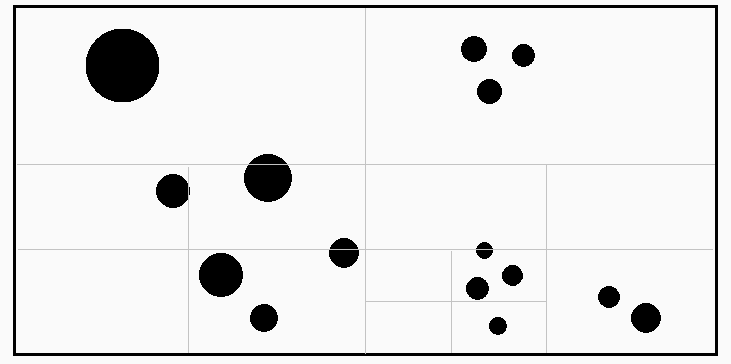
\includegraphics[width=10cm]{img_02.png}
    \end{figure}
\end{frame}

\begin{frame}[fragile]{Просторно индексирање - квадратно стабло}
     \begin{figure}[htp]
        \centering
        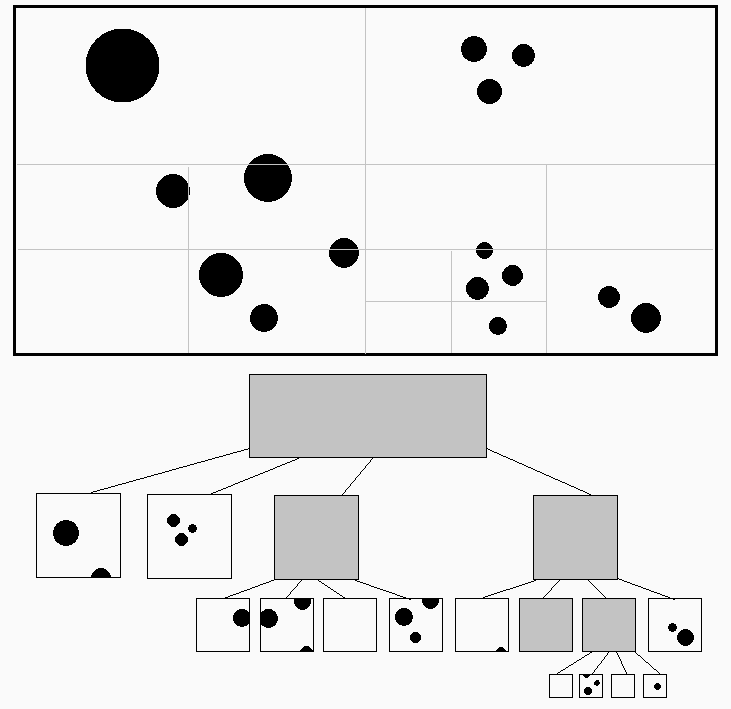
\includegraphics[width=8cm]{img_03.png}
    \end{figure}
\end{frame}

\begin{frame}[fragile]{Просторно индексирање - квадратно стабло}
    \begin{minted}{c++}
struct QuadNode {
    Vec2 pos, size;
    std::vector<PhysBody*> obj;
    QuadNode* child[4];
    unsigned capacity;
}; // naphy/quadtree.h
for (QuadNode& leaf : leaves) {
    std::vector<PhysBody*>* body = leaf->object;
    for (unsigned i = 0; i < body->size; i++) {
        for (unsigned j = i + 1; j < body->size; j++) {
            PhysBody *A = body[i], *B = body[j];
        }
    }
} // naphy/physscene.cpp :: collision_quadtree()
    \end{minted}
\end{frame}

%-------------------------------------------------------------------------------------

\section{Регулисање нумеричких грешака}
\begin{frame}[fragile]{Регулисање нумеричких грешака}
    Коефицијент реституције: $e \in [0, 1]$ \\
    $\lambda = -(1 + e) \cdot \frac{JV}{J M^{-1} J^T}$ \\
    Баумгарте стабилизација: $\beta \in [0, 1], b = \beta \cdot \frac{C}{dt}$ \\
    $\lambda = -(1 + e + b) \frac{JV}{J M^{-1} J^T}$ \\
    Ограничење импулса: $\lambda _{acc}$: $\lambda`_{(i)} = max(\lambda _{acc} + \lambda _{(i)}, 0) - \lambda_{acc}$ \\
    Допуштен упад: деловати импулсом $\lambda_{slop} = \beta_{bias} max(C - \beta_{slop})$
    
    \begin{minted}{c++}
  double slop = 0.07f;
  double bias = 0.6f;
  double correction = bias * max(depth - slop, 0.0);
  Vec2 pcorr = n * correction / (A->m_inv + B->m_inv);
  	
  A->pos -= pcorr * A->m_inv;
  B->pos += pcorr * B->m_inv;
  // naphy/arbiter.cpp :: post_solve()
    \end{minted}
\end{frame}

%-------------------------------------------------------------------------------------

\section{Пример}
\begin{frame}{Пример - тела, арбитери, опруге, квадратно стабло}
    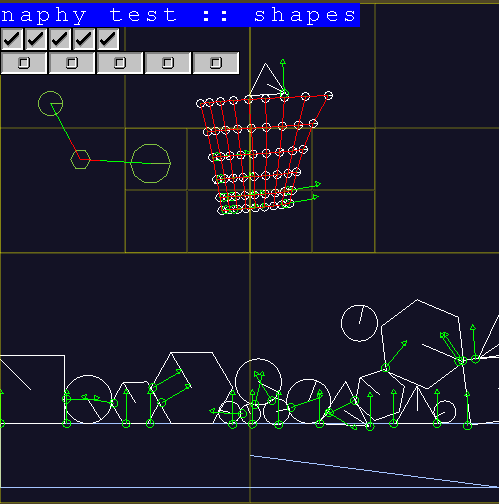
\includegraphics[width=8cm]{ss_01.png}
\end{frame}

\begin{frame}{Пример - нестабилност}
    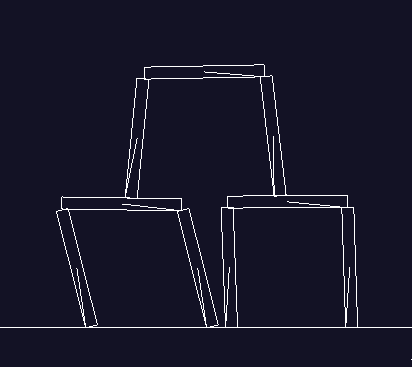
\includegraphics[width=8cm]{ss_02.png}
\end{frame}

\begin{frame}{Пример - нешто конкретније}
    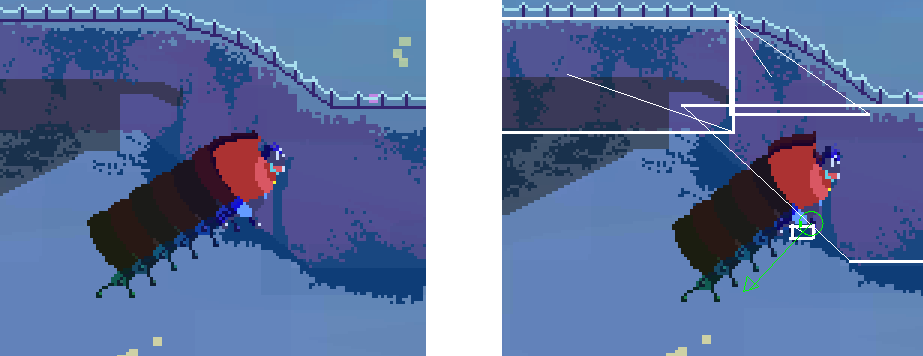
\includegraphics[width=11cm]{ss_03.png}
\end{frame}

%-------------------------------------------------------------------------------------

\section{Литература}
\begin{frame}{Литература}
    \color{blue}
    \underline{\href{https://box2d.org/files/ErinCatto_IterativeDynamics_GDC2005.pdf}{Erin Catto: Iterative Dynamics with Temporal Coherence}} \\
    \underline{\href{https://box2d.org/files/ErinCatto_SequentialImpulses_GDC2006.pdf}{Erin Catto: Fast and Simple Physics using Sequential Impulses}} \\
    \underline{\href{https://box2d.org/files/ErinCatto_SequentialImpulses_GDC2006.pdf}{Erin Catto: Modeling and Solving Constraints}} \\
    \underline{\href{https://github.com/tutsplus/ImpulseEngine}{ImpulseEngine}} \\
    \underline{\href{https://kevinyu.net/2018/02/01/improving-the-stability-of-your-physics/}{Improving the stability of your physics}} \\
    \underline{\href{https://research.ncl.ac.uk/game/mastersdegree/gametechnologies/previousinformation/physics6collisionresponse/2017\%20Tutorial\%206\%20-\%20Collision\%20Response.pdf}{Collision Response}} \\
    \underline{\href{http://allenchou.net/2013/12/game-physics-constraints-sequential-impulse/}{Ming-Lun Chou: Constraints \& Sequential Impulse}}
    
\end{frame}


\end{document}